\documentclass{article}


\usepackage{amsmath} % math stuff
\usepackage{amssymb} % math stuff
\usepackage{array} % equations and stuff
\usepackage{bm} % bold math
%\usepackage{caption} % suppressed table numbering; incompatible with revtex, and longtable, I think
\usepackage{comment} % comment environment
%\usepackage{enumitem} % customization of enumeration, itemize, and description
\usepackage[T1]{fontenc} % font encoding for special characters, must also use scalable font package
\usepackage[margin=0.8in]{geometry} % paper sizes and margins (but be careful not to mess up pre-defined pages)
\usepackage{graphicx} % for graphics
%\usepackage{helvet} % default font is the helvetica postscript font
\usepackage{lipsum} % lorem ipsum filler text
\usepackage{lmodern} % scalable font?
\usepackage{longtable} % multi-page tables
\usepackage{mathrsfs} % math script font
\usepackage{mhchem} % easier chemical formula
\usepackage{microtype} % allows disabling of ligatures
%\usepackage{newcent} % new century schoolbook font
\usepackage{nicefrac}
\usepackage{parskip} % removes paragraph indentation, and adjusts paragraph skip, as well as list items
%\usepackage{setspace} % adjust text spacing and indents
\usepackage{siunitx} % decimal alignment
\usepackage{subfigure} % divided figures
%\usepackage{tabu} % extra table options
\usepackage{textcomp} % symbols
\usepackage{threeparttablex} % better footnotes with longtable
\usepackage{titling} % title placement
\usepackage{ulem} % strikethrough text
%\usepackage{url} % superceded by hyperref
\usepackage{verbatim} % verbatim environment
\usepackage{xcolor} % colors and color boxes
\usepackage{xspace} % commands that don't eat up white space
\usepackage{hyperref} % links and page setup; should always come last

\hypersetup{
	bookmarks=true,
	colorlinks=true,
	citecolor=blue,
	linkcolor=blue,
	urlcolor=blue,
	pdfstartview={XYZ null null 1.0} % default open view is 100%
}

\DisableLigatures[f]{encoding = *, family = * } % disable ff, fi, fl ligatures, without f option, it also disables -- = endash
\renewcommand{\arraystretch}{1} % extra vertical space in tables

\begin{document}

\pagestyle{empty} % don't number pages

% custom title
\begin{center}
{\LARGE Express Riddler}

\vspace{0.15in}

{\Large 31 January 2020}
\end{center}


\section*{Riddle:}

At the recent World Indoor Bowls Championships in Great Yarmouth, England, one of the rolls by Nick Brett went viral.
Here it is in all its glory:

\href{https://twitter.com/SportsCenter/status/1220355057503363072}{Video link}

In order for Nick’s green bowl to split the two red bowls, he needed expert precision in both the speed of the roll and its final angle of approach.

Suppose you were standing in Nick's shoes, and you wanted to split two of your opponent's bowls.
Let's simplify the math a little, and say that each bowl is a sphere with a radius of 1.
Let's further suppose that your opponent's two red bowls are separated by a distance of 3—that is, the centers of the red bowls are separated by a distance of 5.
Define $\phi$ as the angle between the path your bowl is on and the line connecting your opponent's bowls.

For example, here's how you could split your opponent's bowls when $\phi$ is 75 degrees:

\vspace{0.15in}
\begin{center}
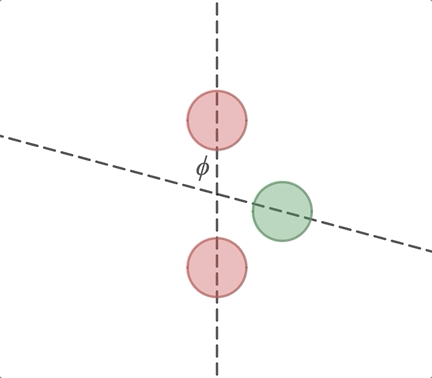
\includegraphics[width=2.5in]{bowls_diagram1.png}
\end{center}
\vspace{0.15in}

What is the \textit{minimum} value of $\phi$ that will allow your bowl to split your opponent's bowls without hitting them?

\section*{Solution:}

This is a pretty basic geometry problem.
I have expanded the above diagram with a few extra labels:

\vspace{0.15in}
\begin{center}
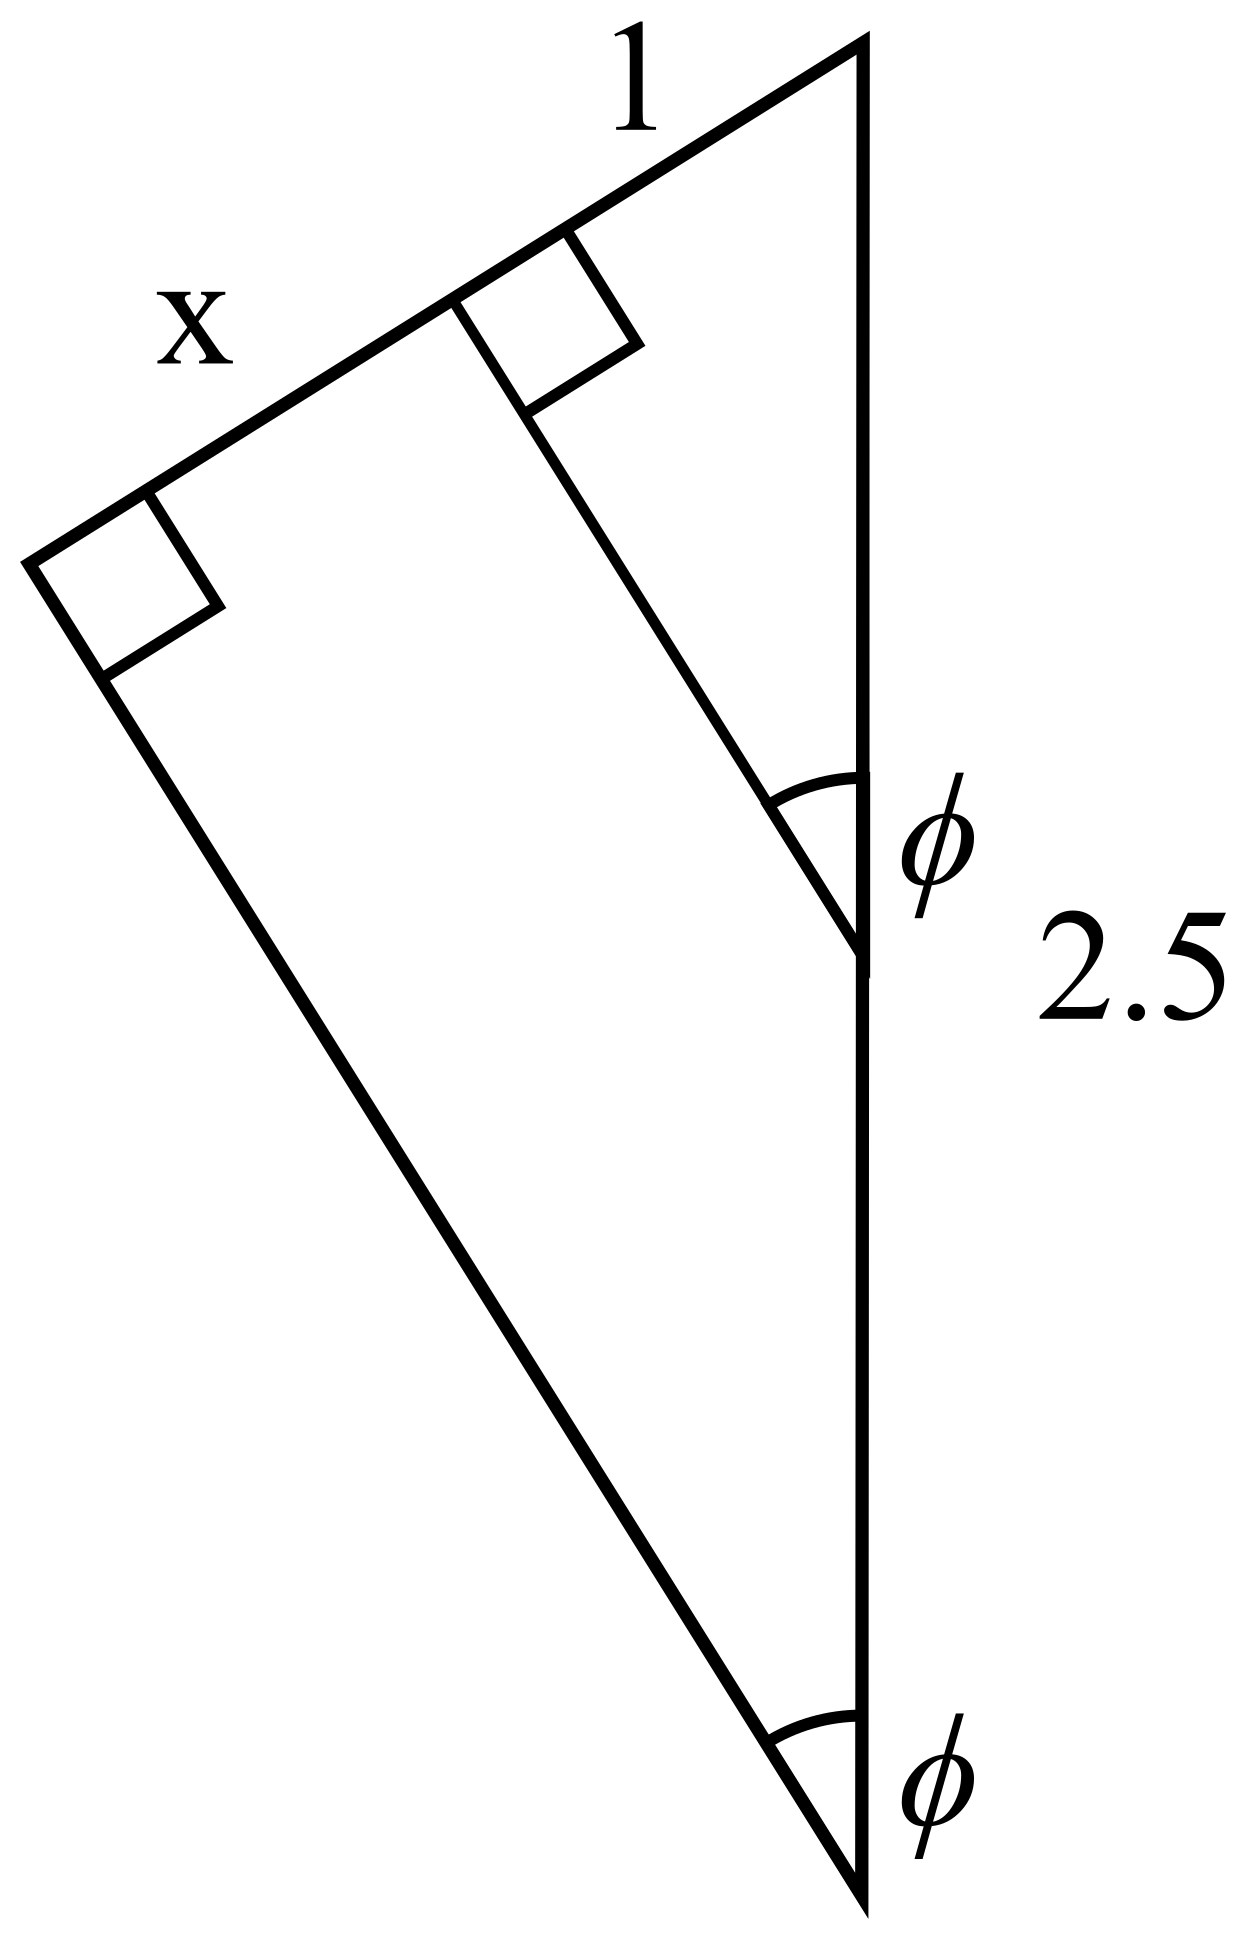
\includegraphics[width=1.5in]{bowls_diagram2.png}
\end{center}
\vspace{0.15in}

Here, $x$ is half the total width available to your bowl, and the vertical distance is 2.5, which is half the distance between the opponent's bowls' centers.
The solution is to solve for $\phi$ when $x=1$, which is easy because (as I highlighted) there is a nice right triangle there.
I just need to solve $\sin(\phi)=\nicefrac{1+x}{2.5}$, or $\phi=\sin^{-1}(0.8)$.
This gives the solution
\fcolorbox{red}{white}{$\phi\approx\ang{53.13}$}\,.



\end{document}